\section{Implementation}
\SectionPage

\begin{frame}
  \frametitle{Module}
  \begin{itemize}
    \pause
    \item A module needs to:
      \pause
      \begin{itemize}
        \item Initialize some state
        \pause
        \item Update the state based on events
        \pause
        \item React to state changes
      \end{itemize}
      \pause
    \item Module architecture is inspired by Elm and MVC
      \pause
    \item A module should be \textit{pure}
  \end{itemize}
\end{frame}

\begin{frame}
  \frametitle{Module example in TypeScript}
  \begin{center}
    \lstinputlisting
    [ language=TypeScript
    ]{./code/module.ts}
  \end{center}
\end{frame}

\begin{frame}
  \frametitle{Counter module example: init}
  \begin{center}
    \lstinputlisting
    [ language=TypeScript
    ]{./code/module-counter-init.ts}
  \end{center}
\end{frame}

\begin{frame}
  \frametitle{Counter module example: handler}
  \begin{center}
    \lstinputlisting
    [ language=TypeScript
    ]{./code/module-counter-handler.ts}
  \end{center}
\end{frame}

%\hidelogo

\begin{frame}
  \frametitle{Module dependencies}
  \begin{figure}
    \centering
      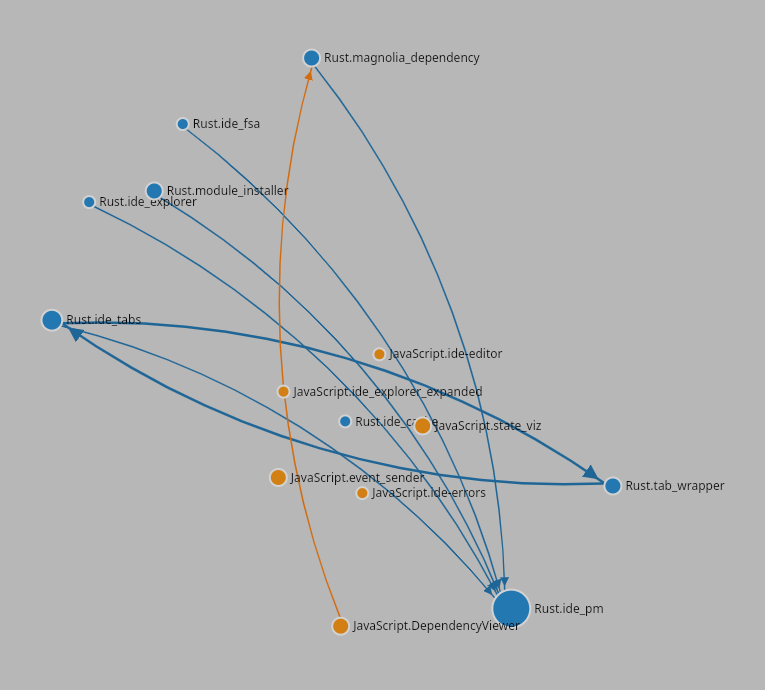
\includegraphics[width=0.7\textwidth]{./pics/module-dependencies.png}
  \end{figure}
\end{frame}

%\showlogo
